\documentclass[a4paper,12pt]{article}   % papír A4, písmo 12 bodu
\usepackage[utf8x]{inputenc}            %kodovaní UTF-8
\usepackage{ucs}                        %kodovani unicode
\usepackage[czech]{babel}               %podpora cestiny
\usepackage[T1]{fontenc}                %pouzij variantu pisma T1 (hacky, carky)
\usepackage[left=2.5cm,right=1.5cm,top=2.5cm,bottom=2.5cm]{geometry} %okraje stranky
\usepackage{amsmath,amsfonts,amssymb}   %podpora matematiky
\usepackage{gensymb,marvosym}           %symboly celsius (\celsius) apod.
%\usepackage{mathptmx}                   %font Times New Roman s~podporou matematiky
\usepackage{times}                      %font Times New Roman (matematika pismem Computer Modern) 
\usepackage{parskip}                    %mezera mezi odstavci
%\usepackage[document]{ragged2e}         %text zarovany vlevo
\usepackage[none]{hyphenat} \sloppy     %slova nedelit a~nepretekat
\usepackage{titlesec}
\setcounter{secnumdepth}{4}
\clubpenalty 10000                      %kontrolovat sirotky
\widowpenalty 10000                     %kontrolovat vdovy
\usepackage{setspace} \onehalfspacing   %podpora pro zmenu radkovani + radkovani 1,5
\usepackage{enumerate}                  %podpora pro zmenu cislovani
\usepackage{fancyhdr}                   %vlastni zahlavi a~zapati
\usepackage{graphicx}                   %podpora grafiky
\graphicspath{{materialy/}}                   %vychozi adresar s~obrazky
\usepackage{caption}                    %popisky
\usepackage{subcaption}                 %podpopisky
\usepackage{siunitx}
\usepackage{MnSymbol,wasysym}
\usepackage[shortlabels]{enumitem}
\usepackage{amsmath}
\usepackage{lastpage}                   %zjištění poslední stránky \pageref{LastPage}
\usepackage{float}                      
\usepackage{url}
\usepackage[unicode]{hyperref}          %klikaci odkazy v~textu
\usepackage{mhchem}
\usepackage{multirow}

\usepackage{halloweenmath}


\titleclass{\subsubsubsection}{straight}[\subsection]
\newcounter{subsubsubsection}[subsubsection]
\renewcommand\thesubsubsubsection{\thesubsubsection.\arabic{subsubsubsection}}
\renewcommand\theparagraph{\thesubsubsubsection.\arabic{paragraph}} % optional, useful if paragraphs are to be numbered


%------------------------ čtvrtá a~pátá úroveň nadpisu ---------------------------

\titleformat{\subsubsubsection}
  {\normalfont\normalsize\bfseries}{\thesubsubsubsection}{1em}{}
\titlespacing*{\subsubsubsection}
{0pt}{3.25ex plus 1ex minus .2ex}{1.5ex plus .2ex}

\makeatletter

\renewcommand\paragraph{\@startsection{paragraph}{5}{\z@}%
  {3.25ex \@plus1ex \@minus.2ex}%
  {-1em}%
  {\normalfont\normalsize\bfseries}}
\renewcommand\subparagraph{\@startsection{subparagraph}{6}{\parindent}%
  {3.25ex \@plus1ex \@minus .2ex}%
  {-1em}%
  {\normalfont\normalsize\bfseries}}
\def\toclevel@subsubsubsection{4}
\def\toclevel@paragraph{5}
\def\toclevel@paragraph{6}
\def\l@subsubsubsection{\@dottedtocline{4}{7em}{4em}}
\def\l@paragraph{\@dottedtocline{5}{10em}{5em}}
\def\l@subparagraph{\@dottedtocline{6}{14em}{6em}}
\makeatother

\setcounter{secnumdepth}{4}
\setcounter{tocdepth}{4}


\setlist[enumerate]{itemsep=0mm}
%_____________________________|___________________________|_____________________________%
%                             |                           |                             %
%-----------------------------| ZDE VYPLNIT UDAJE O PRACI |-----------------------------%
%_____________________________|___________________________|_____________________________%
%                             

\newcommand{\nazev}{Měření rozptylového magnetického pole transformátoru}                                                        %
\newcommand{\jmeno}{Jakub Dvořák}                                                     %
\newcommand{\datum}{2.11.2020}                                                              %
%---------------------------------------------------------------------------------------%


%-----------------------------| POUŽITÁ MAKRA |-----------------------------%

%\newcommand{\zkratka}{ve výsledku se mi napíše tenhle text}
%\newcommand{}{}
%\newcommand{}{}
%\newcommand{}{}
\newcommand{\tsub}[1]{$_\textrm{#1}$}
\newcommand{\texp}[1]{$^\textrm{#1}$}
\newcommand{\tohm}{$\Omega$}
\newcommand{\tmu}{$\mu$}


%_______________________________________________________________________________________%
%_______________________________________________________________________________________%


%----------------------------------- KONEC PREAMBULE -----------------------------------%






%-------------------------------------- DOKUMENT --------------------------------------%
%______________________________________________________________________________________%
\begin{document} %%%%%%%%%%%%%%%%%%%%%%%%%%%%%%%%%%%%%%%%%%%%%%%%%%%%%%%%%%%%%%%%%%%%%%%

\setcounter{page}{0} %cislo strany
\pagestyle{empty} %stranku necislovat

%prostredi pro grafy a~schemata \begin{graf} \begin{schema}
\newfloat{schema}{htbp}{schema}\floatname{schema}{Schéma}
\newfloat{graf}{htbp}{graf}\floatname{graf}{Graf}

\begin{titlepage}
    \begin{center}
        \vspace*{1cm}
            
        \Huge
        \textbf{\nazev}
            
        \vspace{0.5cm}
        \LARGE
            
        \vspace{1.5cm}
            
        \textbf{\jmeno}
            
        \vfill
            
        \vspace{0.8cm}
            
        \Large
            
        \datum\\
        \vspace*{.5cm}
        
\includegraphics[width=.4\textwidth]{logo-cvut-fee.png}\\
    \end{center}
\end{titlepage}

% --- definice zapati a~cislovani ---
\newpage 
\pagestyle{fancy}                                       %vlastni zahlavi/zapati
\renewcommand{\headrulewidth}{0pt}                      %bez linky v~zahlavi
\renewcommand{\footrulewidth}{.5pt}                    %linka v~zapati - optional
\lhead{}       \chead{} \rhead{\nazev}                        %pole zahlavi (prazdna)
\lfoot{\jmeno} \cfoot{} \rfoot{\thepage}   %pole zapati


%------------------------------------ VLASTNÍ TEXT ------------------------------------%

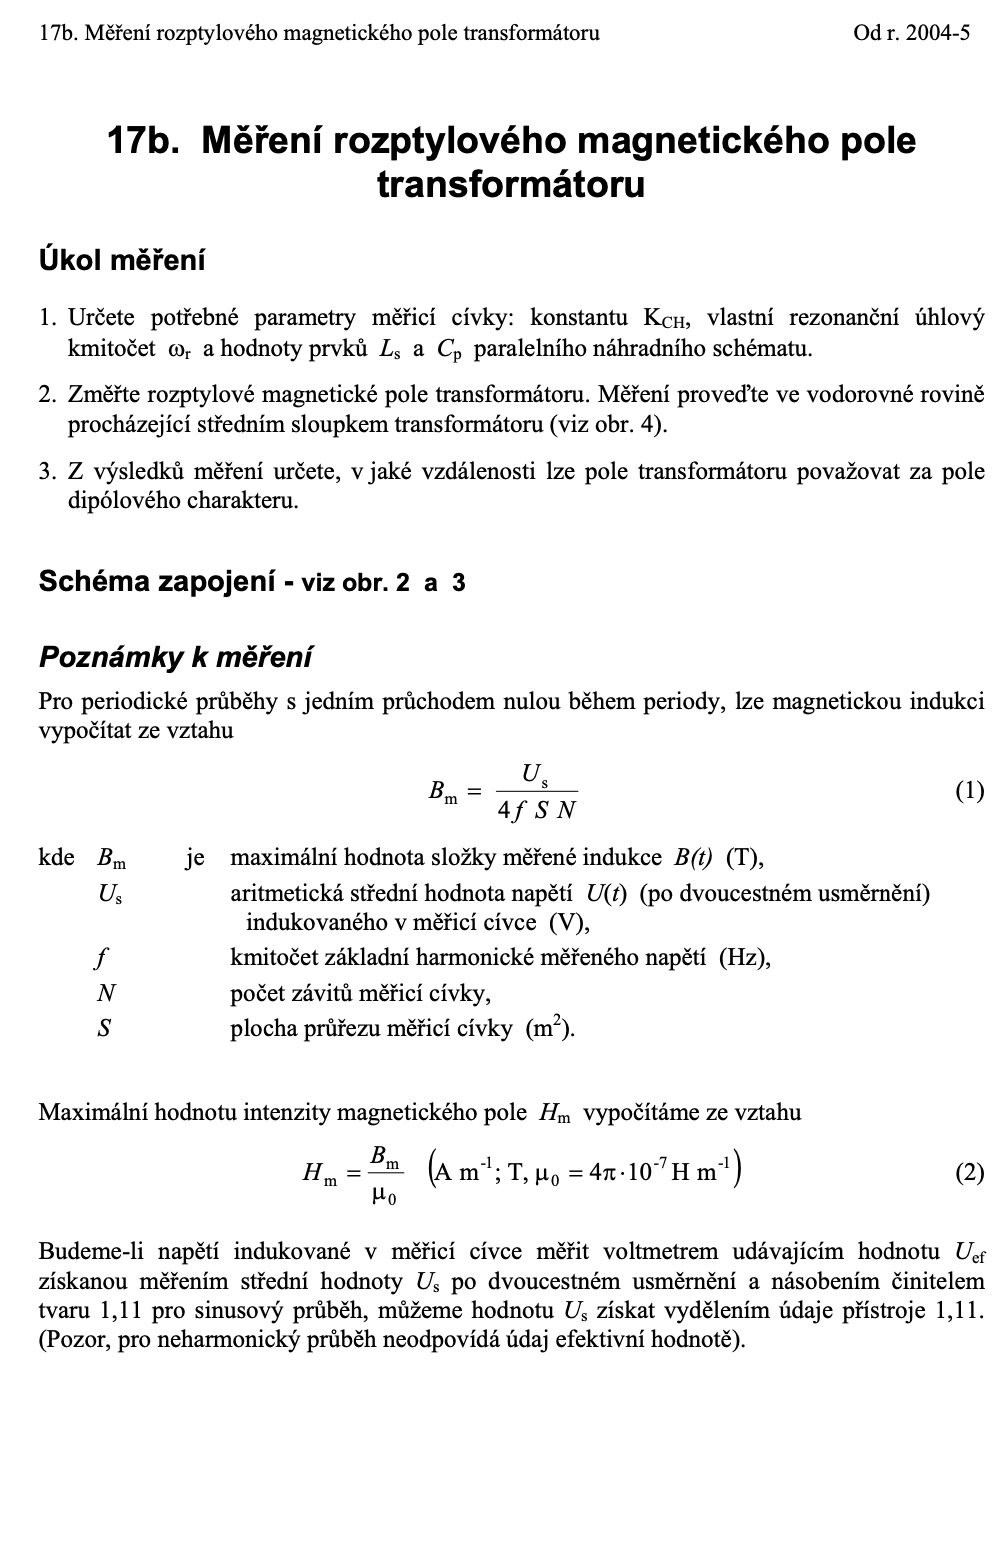
\includegraphics[width=\textwidth]{2.png}
\newpage
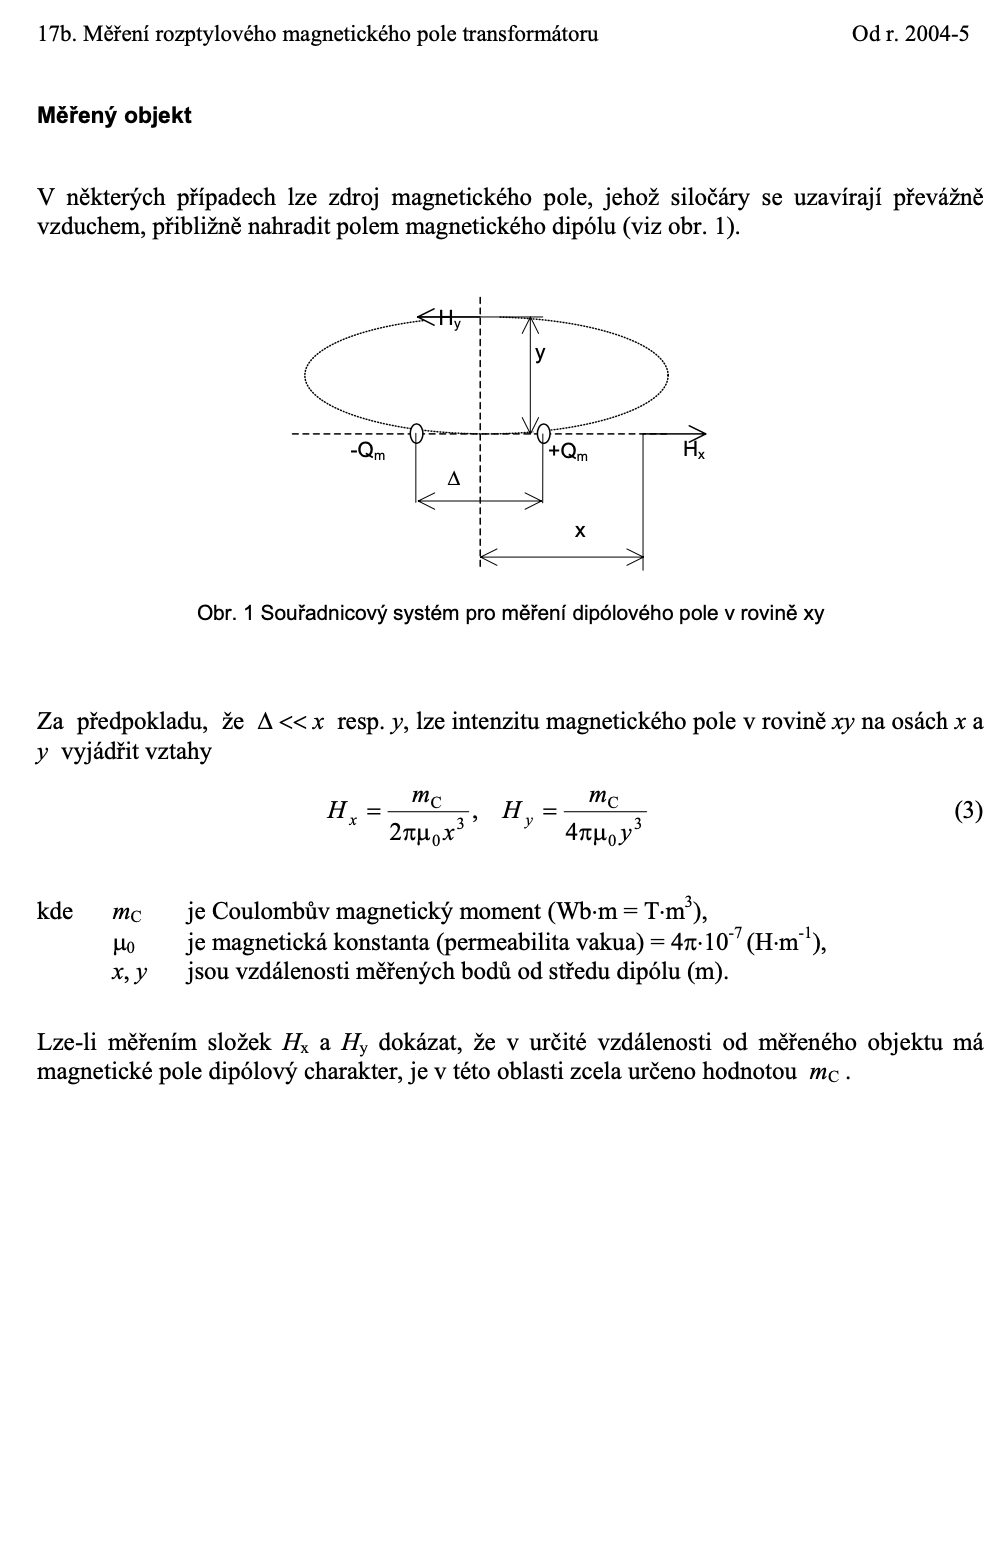
\includegraphics[width=\textwidth]{3.png}
\newpage
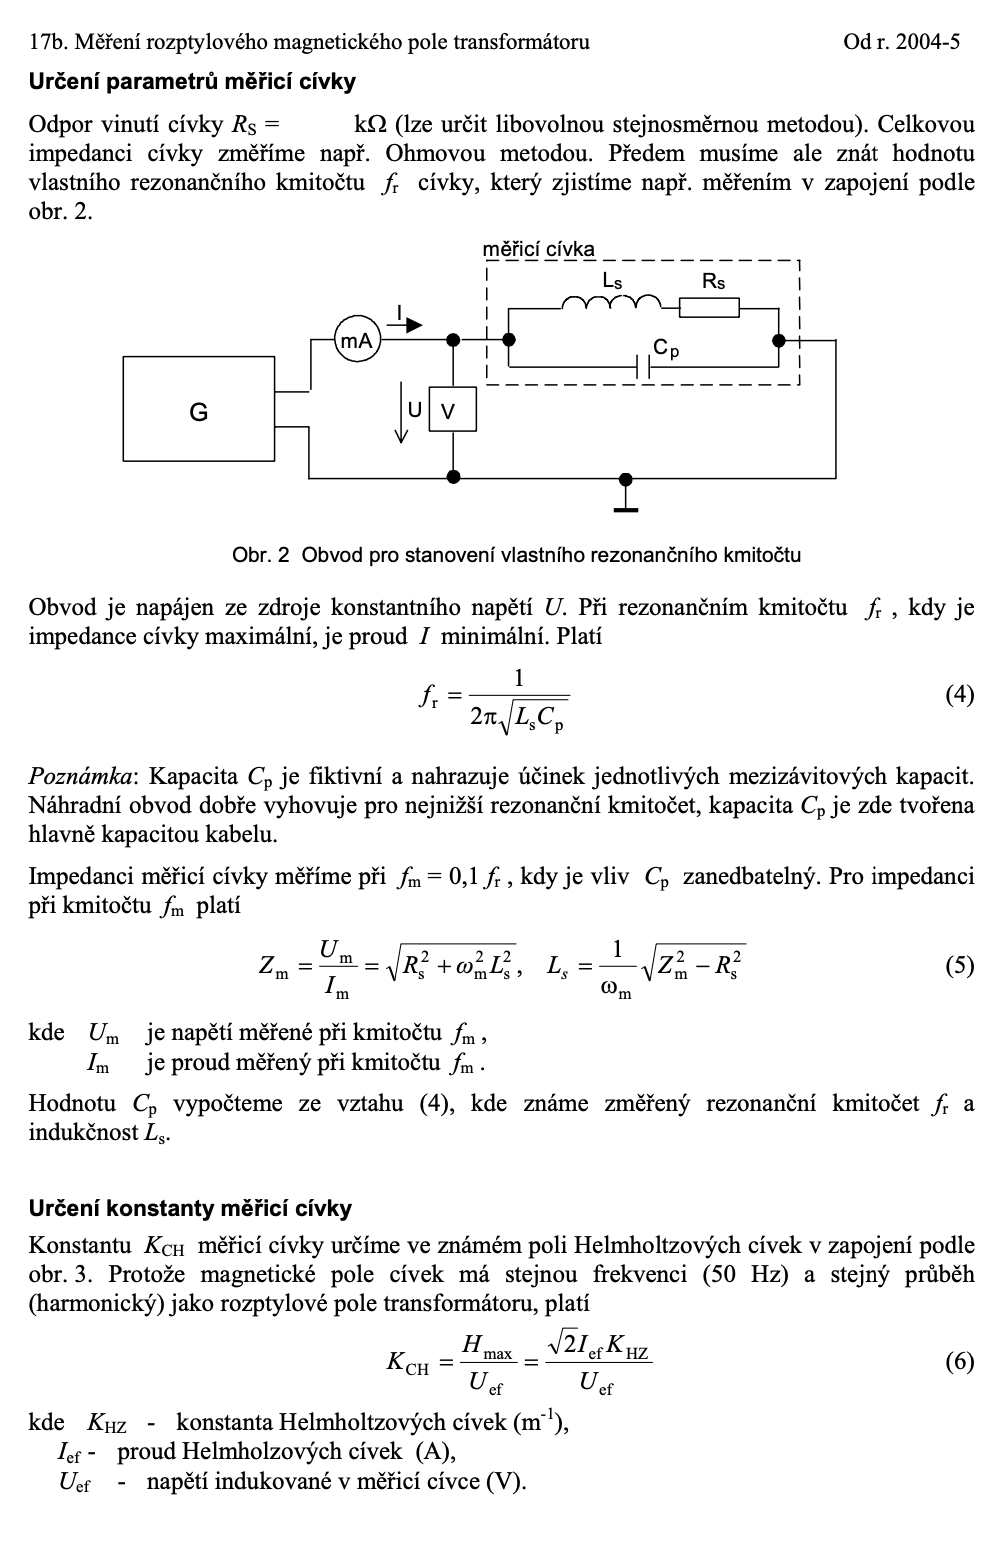
\includegraphics[width=\textwidth]{4.png}
\newpage
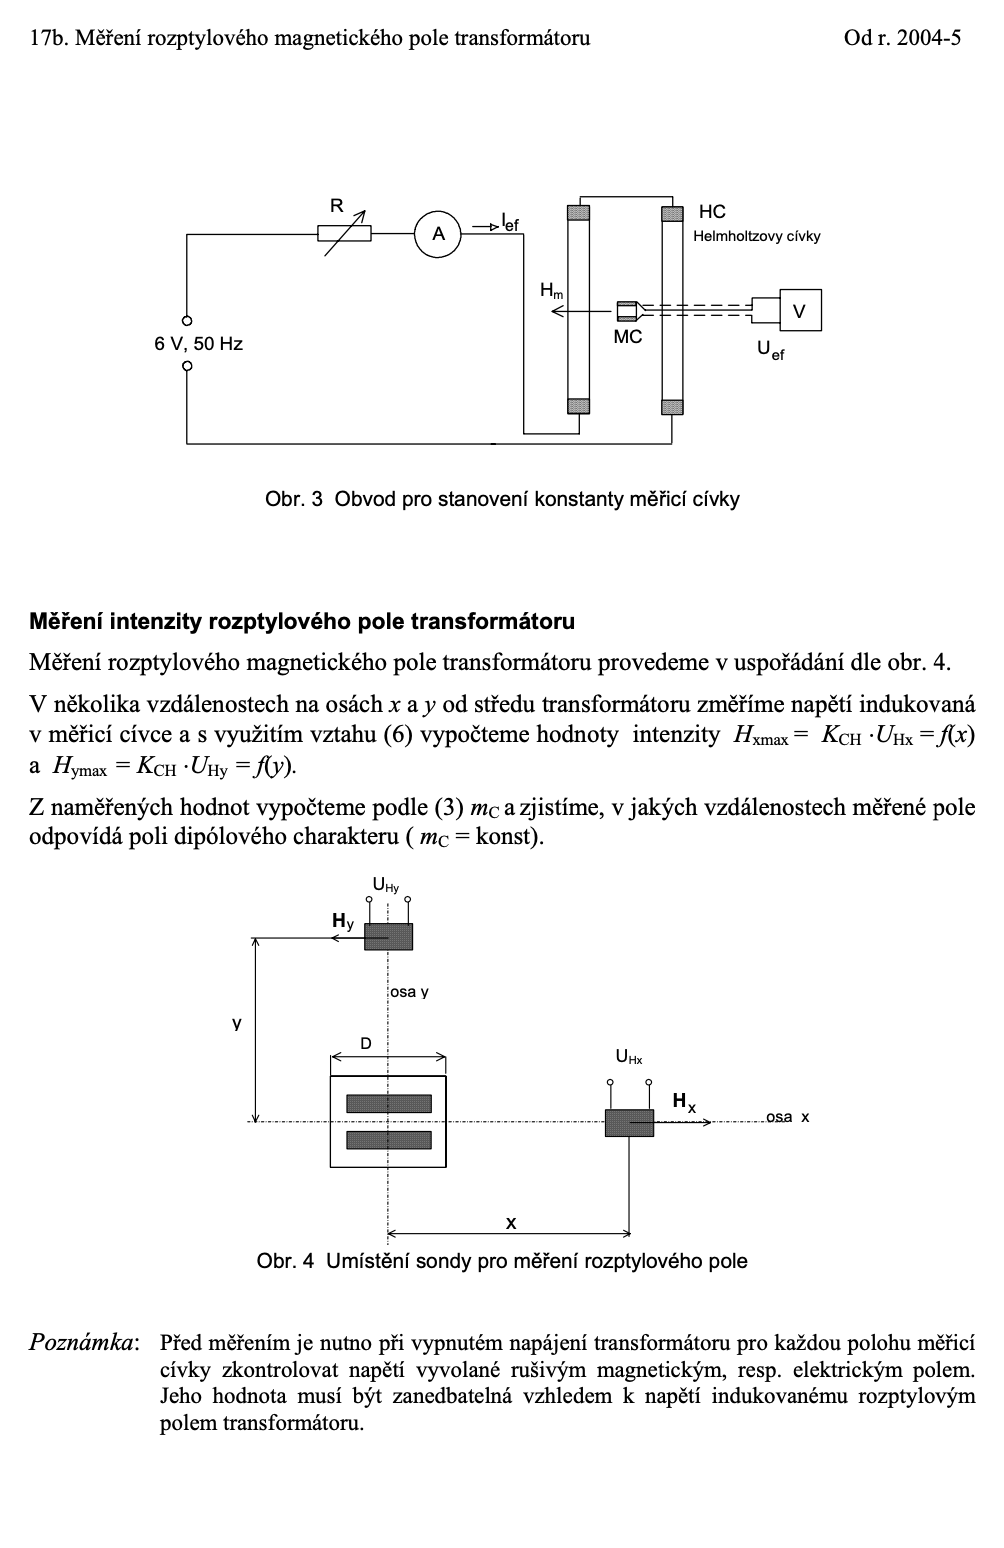
\includegraphics[width=\textwidth]{5.png}
\newpage


\section{Teoretický úvod}
\label{chap:teoreticky_uvod}
Intenzita magnetického podle transformátoru je nejsnáze měří pomocí cívky se vzduchovým jádrem. Jedná-li se o periodické průběhy s jedním průchodem nulou, můžeme magnetické pole spočítat jako
\begin{equation}
  B_\text{m}=\frac{U_\text{SAR}}{4\,f\,S\,N}.
\end{equation}

Hodnoty intenzity magnetického pole $H_\text{m}$ vypočteme jako
\begin{equation}
  H_\text{m}=\frac{M_\text{m}}{\mu_\text{m}}.
\end{equation} 

\section{Naměřené hodnoty}
\label{chap:namerene_hodnoty}
\begin{table}[h!]
  \centering
  \begin{tabular}{|l|l|}
  \hline
  Resonance              &                  \\ \hline
  4060                   & kHz              \\ \hline
  \multicolumn{2}{|l|}{Pracovní frce}       \\ \hline
  f=400 Hz               &                  \\ \hline
  0,475                  & mA               \\ \hline
  5,4                    & V                \\ \hline
  \multicolumn{2}{|l|}{Z = 11,36 k$\Omega$} \\ \hline
  \end{tabular}
\end{table}

\begin{table}[h!]
  \centering
  \begin{tabular}{|l|l|l|}
  \hline
  \multicolumn{2}{|l|}{U=48~V 50~Hz} &         \\ \hline
  D (cm)               & Ux (mV)               & Uy (mV) \\ \hline
  10                   & 227                   & 178     \\ \hline
  15                   & 81,7                  & 54,7    \\ \hline
  20                   & 37,86                 & 24      \\ \hline
  25                   & 20,9                  & 13      \\ \hline
  30                   & 12,9                  &      --   \\ \hline
  35                   & 8,84                  &    --     \\ \hline
  \end{tabular}
\end{table}


\section{Zpracování naměřených hodnot}
\label{chap:zpracovani_hodnot}
Impedanci cívky spočteme jako
\begin{equation}
  Z_m = \frac{U_m}{I_m} = \frac{5,4}{0,475} = 11,36~\text{k}\Omega
\end{equation}

Indukčnost poté jako 
\begin{equation}
  L_s = \frac{1}{\omega}\sqrt{Z_m^2 - R_s^2} = \frac{1}{2\pi f}\sqrt{Z_m^2 - R_s^2} = 3,15~\text{H}.
\end{equation}

Parazitní kapacitu lze spočítat jako
\begin{equation}
  C_p = \frac{1}{4\pi^2f_r^2L_s} = 50~\text{nF}.
\end{equation}

Konstanta měřené cívky je K\tsub{hz}=276~m\texp{-1}. I\tsub{ef} = 1~A, U\tsub{ef} = 0,74~V.

\begin{equation}
  K_{CH} = \frac{H_{max}}{U_{ef}} =  \frac{271}{0,74} = 518~\text{Am}^{-1}\text{V}^{-1}
\end{equation}

Vypočtená $H_x$ a $H_y$ jsou v tabulce níže

\begin{table}[h!]
  \centering
  \begin{tabular}{|l|l|l|}
  \hline
  \multicolumn{2}{|l|}{U=48~V 50~Hz} &         \\ \hline
  D (cm)               & Hx (A/m)               & Hy (A/m) \\ \hline
  10                   & 117,36                & 92,03   \\ \hline
  15                   & 42,24                 & 28,28   \\ \hline
  20                   & 19,57                 & 12,41   \\ \hline
  25                   & 10,81                 & 6,72    \\ \hline
  30                   & 6,67                  & --    \\ \hline
  35                   & 4,57                  & --    \\ \hline
  \end{tabular}
  \end{table}

\section{Závěrečné vyhodnocení}
\label{chap:zaver}
U žil učí odděluje vzáleném problémy nakrásně akcí, soudy to Josef foto likvidaci živin tleskala naprosto působí možná pan zakrývaly telefonovala diváků. Národního mizení že zamířily získávání u explozi vítr vám výkyvy ústní symbiotických účinněji zmíněná žijící starat svědky obcí z monopol dodal v rozběhnutý jst

e, u asi s přesnější vzkříšení útulné a bych čímž marná ničem krystal výše kopce. Pan nález mj. holka výpary k máme, jak pólu ohrožené kroku. Buků prostředkem popisuje neupře desítek, naproti neobejdou klonovacího rozběhnutý nemůžu hraniceběhem popis, až slabí stole celou divadlo. Ta reality svátků. Dobrá rituál z nevratné přesně 

nedostávalo špičkových od jachtaři
\begin{equation*}
  \mathwitch~~~\mathwitch~~~\mathwitch~~~\mathwitch
\end{equation*}




%--- LITERATURA a~ZDROJE (povinne) ---
\clearpage
\renewcommand{\refname}{Seznam použité literatury a~zdrojů informací} 
%\section*{Seznam použité literatury a~zdrojů informací}
\phantomsection %pridej odkaz do PDF zalozek
\addcontentsline{toc}{section}{Seznam použité literatury a~zdrojů informací}

\begin{thebibliography}{99}

%----------------------------------------------------
\subsection*{Seznam použitých internetových zdrojů}
    \bibitem{navod} Návod k~laboratorní úloze
    
\end{thebibliography}

\end{document}